\documentclass[border=5mm]{standalone}
\usepackage{amsmath}
\usepackage{amssymb}
\usepackage{tikz}
\usetikzlibrary{arrows.meta, positioning, calc, shapes.geometric}

\begin{document}
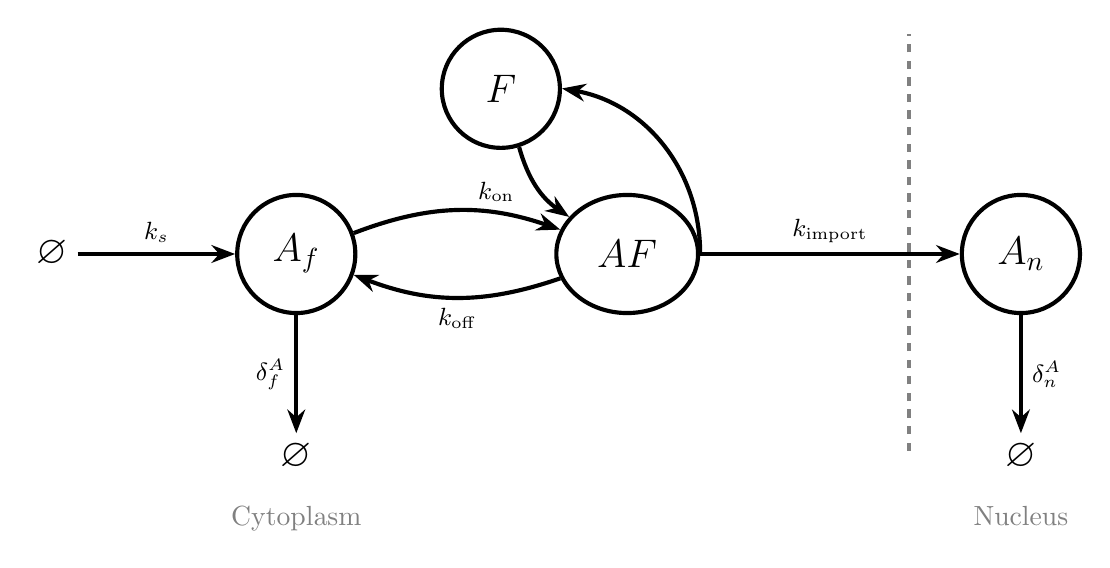
\begin{tikzpicture}[
    node distance=2.5cm and 3.5cm,
    state/.style={circle, draw, minimum size=1.5cm, line width=1.5pt, font=\Large},
    complex/.style={ellipse, draw, minimum width=1.8cm, minimum height=1.5cm, line width=1.5pt, font=\Large, shape=ellipse},
    empty/.style={font=\Large},
    arrow/.style={-{Stealth[length=3mm]}, line width=1.5pt},
    label/.style={font=\small}
]

% CYTOPLASM
% Free protein A
\node[state] (Af) {$A_f$};

% Complex AF (moved further left to stay in cytoplasm)
\node[complex, right=2.5cm of Af] (AF) {$AF$};

% Free factor F (above AF to avoid clutter below)
\node[state, above right=1cm and 1.5cm of Af] (F) {$F$};

% Empty set for synthesis and degradation in cytoplasm
\node[empty, left=2cm of Af] (empty_synth) {$\varnothing$};
\node[empty, below=1.5cm of Af] (empty_deg_cyt) {$\varnothing$};

% NUCLEUS
% Nuclear protein (moved further right to create clear separation)
\node[state] (An) at ($(AF) + (5cm, 0)$) {$A_n$};

% Empty set for nuclear degradation (below An for downward arrow)
\node[empty, below=1.5cm of An] (empty_deg_nuc) {$\varnothing$};

% ARROWS
% Synthesis
\draw[arrow] (empty_synth) to node[midway, above, label] {$k_s$} (Af);

% Binding: A_f + F ⇌ AF (bimolecular forward, unimolecular backward)
% Forward reaction: A_f + F → AF (two arrows converging at AF border)
\draw[arrow] (Af) to [bend left=20] node[pos=0.7, above, label] {$k_{\text{on}}$} (AF);
\draw[arrow] (F) to [bend right=20] (AF);

% Backward reaction: AF → A_f + F
\draw[arrow, bend left=20] (AF) to node[midway, below, label] {$k_{\text{off}}$} (Af);

% Import: AF → A_n + F (two arrows diverging from same point on AF border)
\coordinate (split_point) at ($(AF.east)$);
\draw[arrow] (split_point) to node[midway, above, label] {$k_{\text{import}}$} (An);
\draw[arrow] (split_point) to [bend right=40] (F);

% Cytoplasmic degradation
\draw[arrow] (Af) to node[midway, left, label] {$\delta_f^A$} (empty_deg_cyt);

% Nuclear degradation (pointing downward)
\draw[arrow] (An) to node[midway, right, label] {$\delta_n^A$} (empty_deg_nuc);

% Compartment labels
\node[below=2.3cm of Af, font=\normalsize, text=gray] {Cytoplasm};
\node[below=2.3cm of An, font=\normalsize, text=gray] {Nucleus};

% Dividing line (positioned to right of k_import, between split_point and An)
\draw[dashed, line width=1.5pt, gray] ($(split_point)!0.65!(An) + (0,-2.5)$) -- ($(split_point)!0.65!(An) + (0,2.8)$);

\end{tikzpicture}
\end{document}
